\documentclass[12pt]{article}

%packages
%\usepackage{latexsym}
\usepackage{graphicx}
\usepackage{color}
\usepackage{amsmath}
\usepackage{dsfont}
\usepackage{placeins}
\usepackage{amssymb}
\usepackage{wasysym}
\usepackage{abstract}
\usepackage{hyperref}
\usepackage{etoolbox}
\usepackage{datetime}
\usepackage{xcolor}
\usepackage{alphalph}
\settimeformat{ampmtime}

%\usepackage{pstricks,pst-node,pst-tree}

%\usepackage{algpseudocode}
%\usepackage{amsthm}
%\usepackage{hyperref}
%\usepackage{mathrsfs}
%\usepackage{amsfonts}
%\usepackage{bbding}
%\usepackage{listings}
%\usepackage{appendix}
\usepackage[margin=1in]{geometry}
%\geometry{papersize={8.5in,11in},total={6.5in,9in}}
%\usepackage{cancel}
%\usepackage{algorithmic, algorithm}

\makeatletter
\def\maxwidth{ %
  \ifdim\Gin@nat@width>\linewidth
    \linewidth
  \else
    \Gin@nat@width
  \fi
}
\makeatother

\definecolor{fgcolor}{rgb}{0.345, 0.345, 0.345}
\newcommand{\hlnum}[1]{\textcolor[rgb]{0.686,0.059,0.569}{#1}}%
\newcommand{\hlstr}[1]{\textcolor[rgb]{0.192,0.494,0.8}{#1}}%
\newcommand{\hlcom}[1]{\textcolor[rgb]{0.678,0.584,0.686}{\textit{#1}}}%
\newcommand{\hlopt}[1]{\textcolor[rgb]{0,0,0}{#1}}%
\newcommand{\hlstd}[1]{\textcolor[rgb]{0.345,0.345,0.345}{#1}}%
\newcommand{\hlkwa}[1]{\textcolor[rgb]{0.161,0.373,0.58}{\textbf{#1}}}%
\newcommand{\hlkwb}[1]{\textcolor[rgb]{0.69,0.353,0.396}{#1}}%
\newcommand{\hlkwc}[1]{\textcolor[rgb]{0.333,0.667,0.333}{#1}}%
\newcommand{\hlkwd}[1]{\textcolor[rgb]{0.737,0.353,0.396}{\textbf{#1}}}%

\usepackage{framed}
\makeatletter
\newenvironment{kframe}{%
 \def\at@end@of@kframe{}%
 \ifinner\ifhmode%
  \def\at@end@of@kframe{\end{minipage}}%
  \begin{minipage}{\columnwidth}%
 \fi\fi%
 \def\FrameCommand##1{\hskip\@totalleftmargin \hskip-\fboxsep
 \colorbox{shadecolor}{##1}\hskip-\fboxsep
     % There is no \\@totalrightmargin, so:
     \hskip-\linewidth \hskip-\@totalleftmargin \hskip\columnwidth}%
 \MakeFramed {\advance\hsize-\width
   \@totalleftmargin\z@ \linewidth\hsize
   \@setminipage}}%
 {\par\unskip\endMakeFramed%
 \at@end@of@kframe}
\makeatother

\definecolor{shadecolor}{rgb}{.77, .77, .77}
\definecolor{messagecolor}{rgb}{0, 0, 0}
\definecolor{warningcolor}{rgb}{1, 0, 1}
\definecolor{errorcolor}{rgb}{1, 0, 0}
\newenvironment{knitrout}{}{} % an empty environment to be redefined in TeX

\usepackage{alltt}
\usepackage[T1]{fontenc}

\newcommand{\qu}[1]{``#1''}
\newcounter{probnum}
\setcounter{probnum}{1}

%create definition to allow local margin changes
\def\changemargin#1#2{\list{}{\rightmargin#2\leftmargin#1}\item[]}
\let\endchangemargin=\endlist 

%allow equations to span multiple pages
\allowdisplaybreaks

%define colors and color typesetting conveniences
\definecolor{gray}{rgb}{0.5,0.5,0.5}
\definecolor{black}{rgb}{0,0,0}
\definecolor{white}{rgb}{1,1,1}
\definecolor{blue}{rgb}{0.5,0.5,1}
\newcommand{\inblue}[1]{\color{blue}#1 \color{black}}
\definecolor{green}{rgb}{0.133,0.545,0.133}
\newcommand{\ingreen}[1]{\color{green}#1 \color{black}}
\definecolor{yellow}{rgb}{1,1,0}
\newcommand{\inyellow}[1]{\color{yellow}#1 \color{black}}
\definecolor{orange}{rgb}{0.9,0.649,0}
\newcommand{\inorange}[1]{\color{orange}#1 \color{black}}
\definecolor{red}{rgb}{1,0.133,0.133}
\newcommand{\inred}[1]{\color{red}#1 \color{black}}
\definecolor{purple}{rgb}{0.58,0,0.827}
\newcommand{\inpurple}[1]{\color{purple}#1 \color{black}}
\definecolor{backgcode}{rgb}{0.97,0.97,0.8}
\definecolor{Brown}{cmyk}{0,0.81,1,0.60}
\definecolor{OliveGreen}{cmyk}{0.64,0,0.95,0.40}
\definecolor{CadetBlue}{cmyk}{0.62,0.57,0.23,0}

%define new math operators
\DeclareMathOperator*{\argmax}{arg\,max~}
\DeclareMathOperator*{\argmin}{arg\,min~}
\DeclareMathOperator*{\argsup}{arg\,sup~}
\DeclareMathOperator*{\arginf}{arg\,inf~}
\DeclareMathOperator*{\convolution}{\text{\Huge{$\ast$}}}
\newcommand{\infconv}[2]{\convolution^\infty_{#1 = 1} #2}
%true functions

%%%% GENERAL SHORTCUTS

%shortcuts for pure typesetting conveniences
\newcommand{\bv}[1]{\boldsymbol{#1}}

%shortcuts for compound constants
\newcommand{\BetaDistrConst}{\dfrac{\Gamma(\alpha + \beta)}{\Gamma(\alpha)\Gamma(\beta)}}
\newcommand{\NormDistrConst}{\dfrac{1}{\sqrt{2\pi\sigma^2}}}

%shortcuts for conventional symbols
\newcommand{\tsq}{\tau^2}
\newcommand{\tsqh}{\hat{\tau}^2}
\newcommand{\sigsq}{\sigma^2}
\newcommand{\sigsqsq}{\parens{\sigma^2}^2}
\newcommand{\sigsqovern}{\dfrac{\sigsq}{n}}
\newcommand{\tausq}{\tau^2}
\newcommand{\tausqalpha}{\tau^2_\alpha}
\newcommand{\tausqbeta}{\tau^2_\beta}
\newcommand{\tausqsigma}{\tau^2_\sigma}
\newcommand{\betasq}{\beta^2}
\newcommand{\sigsqvec}{\bv{\sigma}^2}
\newcommand{\sigsqhat}{\hat{\sigma}^2}
\newcommand{\sigsqhatmlebayes}{\sigsqhat_{\text{Bayes, MLE}}}
\newcommand{\sigsqhatmle}[1]{\sigsqhat_{#1, \text{MLE}}}
\newcommand{\bSigma}{\bv{\Sigma}}
\newcommand{\bSigmainv}{\bSigma^{-1}}
\newcommand{\thetavec}{\bv{\theta}}
\newcommand{\thetahat}{\hat{\theta}}
\newcommand{\thetahatmle}{\hat{\theta}_{\mathrm{MLE}}}
\newcommand{\thetavechatmle}{\hat{\thetavec}_{\mathrm{MLE}}}
\newcommand{\muhat}{\hat{\mu}}
\newcommand{\musq}{\mu^2}
\newcommand{\muvec}{\bv{\mu}}
\newcommand{\muhatmle}{\muhat_{\text{MLE}}}
\newcommand{\lambdahat}{\hat{\lambda}}
\newcommand{\lambdahatmle}{\lambdahat_{\text{MLE}}}
\newcommand{\etavec}{\bv{\eta}}
\newcommand{\alphavec}{\bv{\alpha}}
\newcommand{\minimaxdec}{\delta^*_{\mathrm{mm}}}
\newcommand{\ybar}{\bar{y}}
\newcommand{\xbar}{\bar{x}}
\newcommand{\Xbar}{\bar{X}}
\newcommand{\phat}{\hat{p}}
\newcommand{\Phat}{\hat{P}}
\newcommand{\Zbar}{\bar{Z}}
\newcommand{\iid}{~{\buildrel iid \over \sim}~}
\newcommand{\inddist}{~{\buildrel ind \over \sim}~}
\newcommand{\approxdist}{~{\buildrel approx \over \sim}~}
\newcommand{\equalsindist}{~{\buildrel d \over =}~}
\newcommand{\loglik}[1]{\ell\parens{#1}}
\newcommand{\thetahatkminone}{\thetahat^{(k-1)}}
\newcommand{\thetahatkplusone}{\thetahat^{(k+1)}}
\newcommand{\thetahatk}{\thetahat^{(k)}}
\newcommand{\half}{\frac{1}{2}}
\newcommand{\third}{\frac{1}{3}}
\newcommand{\twothirds}{\frac{2}{3}}
\newcommand{\fourth}{\frac{1}{4}}
\newcommand{\fifth}{\frac{1}{5}}
\newcommand{\sixth}{\frac{1}{6}}

%shortcuts for vector and matrix notation
\newcommand{\A}{\bv{A}}
\newcommand{\At}{\A^T}
\newcommand{\Ainv}{\inverse{\A}}
\newcommand{\B}{\bv{B}}
\newcommand{\K}{\bv{K}}
\newcommand{\Kt}{\K^T}
\newcommand{\Kinv}{\inverse{K}}
\newcommand{\Kinvt}{(\Kinv)^T}
\newcommand{\M}{\bv{M}}
\newcommand{\Bt}{\B^T}
\newcommand{\Q}{\bv{Q}}
\newcommand{\Qt}{\Q^T}
\newcommand{\R}{\bv{R}}
\newcommand{\Rt}{\R^T}
\newcommand{\Z}{\bv{Z}}
\newcommand{\X}{\bv{X}}
\newcommand{\Xsub}{\X_{\text{(sub)}}}
\newcommand{\Xsubadj}{\X_{\text{(sub,adj)}}}
\newcommand{\I}{\bv{I}}
\newcommand{\Y}{\bv{Y}}
\newcommand{\sigsqI}{\sigsq\I}
\renewcommand{\P}{\bv{P}}
\newcommand{\Psub}{\P_{\text{(sub)}}}
\newcommand{\Pt}{\P^T}
\newcommand{\Pii}{P_{ii}}
\newcommand{\Pij}{P_{ij}}
\newcommand{\IminP}{(\I-\P)}
\newcommand{\Xt}{\bv{X}^T}
\newcommand{\XtX}{\Xt\X}
\newcommand{\XtXinv}{\parens{\Xt\X}^{-1}}
\newcommand{\XtXinvXt}{\XtXinv\Xt}
\newcommand{\XXtXinvXt}{\X\XtXinvXt}
\newcommand{\x}{\bv{x}}
\newcommand{\onevec}{\bv{1}}
\newcommand{\oneton}{1, \ldots, n}
\newcommand{\yoneton}{y_1, \ldots, y_n}
\newcommand{\yonetonorder}{y_{(1)}, \ldots, y_{(n)}}
\newcommand{\Yoneton}{Y_1, \ldots, Y_n}
\newcommand{\iinoneton}{i \in \braces{\oneton}}
\newcommand{\onetom}{1, \ldots, m}
\newcommand{\jinonetom}{j \in \braces{\onetom}}
\newcommand{\xoneton}{x_1, \ldots, x_n}
\newcommand{\Xoneton}{X_1, \ldots, X_n}
\newcommand{\xt}{\x^T}
\newcommand{\y}{\bv{y}}
\newcommand{\yt}{\y^T}
\renewcommand{\c}{\bv{c}}
\newcommand{\ct}{\c^T}
\newcommand{\tstar}{\bv{t}^*}
\renewcommand{\u}{\bv{u}}
\renewcommand{\v}{\bv{v}}
\renewcommand{\a}{\bv{a}}
\newcommand{\s}{\bv{s}}
\newcommand{\yadj}{\y_{\text{(adj)}}}
\newcommand{\xjadj}{\x_{j\text{(adj)}}}
\newcommand{\xjadjM}{\x_{j \perp M}}
\newcommand{\yhat}{\hat{\y}}
\newcommand{\yhatsub}{\yhat_{\text{(sub)}}}
\newcommand{\yhatstar}{\yhat^*}
\newcommand{\yhatstarnew}{\yhatstar_{\text{new}}}
\newcommand{\z}{\bv{z}}
\newcommand{\zt}{\z^T}
\newcommand{\bb}{\bv{b}}
\newcommand{\bbt}{\bb^T}
\newcommand{\bbeta}{\bv{\beta}}
\newcommand{\beps}{\bv{\epsilon}}
\newcommand{\bepst}{\beps^T}
\newcommand{\e}{\bv{e}}
\newcommand{\Mofy}{\M(\y)}
\newcommand{\KofAlpha}{K(\alpha)}
\newcommand{\ellset}{\mathcal{L}}
\newcommand{\oneminalph}{1-\alpha}
\newcommand{\SSE}{\text{SSE}}
\newcommand{\SSEsub}{\text{SSE}_{\text{(sub)}}}
\newcommand{\MSE}{\text{MSE}}
\newcommand{\RMSE}{\text{RMSE}}
\newcommand{\SSR}{\text{SSR}}
\newcommand{\SST}{\text{SST}}
\newcommand{\JSest}{\delta_{\text{JS}}(\x)}
\newcommand{\Bayesest}{\delta_{\text{Bayes}}(\x)}
\newcommand{\EmpBayesest}{\delta_{\text{EmpBayes}}(\x)}
\newcommand{\BLUPest}{\delta_{\text{BLUP}}}
\newcommand{\MLEest}[1]{\hat{#1}_{\text{MLE}}}

%shortcuts for Linear Algebra stuff (i.e. vectors and matrices)
\newcommand{\twovec}[2]{\bracks{\begin{array}{c} #1 \\ #2 \end{array}}}
\newcommand{\threevec}[3]{\bracks{\begin{array}{c} #1 \\ #2 \\ #3 \end{array}}}
\newcommand{\fivevec}[5]{\bracks{\begin{array}{c} #1 \\ #2 \\ #3 \\ #4 \\ #5 \end{array}}}
\newcommand{\twobytwomat}[4]{\bracks{\begin{array}{cc} #1 & #2 \\ #3 & #4 \end{array}}}
\newcommand{\threebytwomat}[6]{\bracks{\begin{array}{cc} #1 & #2 \\ #3 & #4 \\ #5 & #6 \end{array}}}

%shortcuts for conventional compound symbols
\newcommand{\thetainthetas}{\theta \in \Theta}
\newcommand{\reals}{\mathbb{R}}
\newcommand{\complexes}{\mathbb{C}}
\newcommand{\rationals}{\mathbb{Q}}
\newcommand{\integers}{\mathbb{Z}}
\newcommand{\naturals}{\mathbb{N}}
\newcommand{\forallninN}{~~\forall n \in \naturals}
\newcommand{\forallxinN}[1]{~~\forall #1 \in \reals}
\newcommand{\matrixdims}[2]{\in \reals^{\,#1 \times #2}}
\newcommand{\inRn}[1]{\in \reals^{\,#1}}
\newcommand{\mathimplies}{\quad\Rightarrow\quad}
\newcommand{\mathlogicequiv}{\quad\Leftrightarrow\quad}
\newcommand{\eqncomment}[1]{\quad \text{(#1)}}
\newcommand{\limitn}{\lim_{n \rightarrow \infty}}
\newcommand{\limitN}{\lim_{N \rightarrow \infty}}
\newcommand{\limitd}{\lim_{d \rightarrow \infty}}
\newcommand{\limitt}{\lim_{t \rightarrow \infty}}
\newcommand{\limitsupn}{\limsup_{n \rightarrow \infty}~}
\newcommand{\limitinfn}{\liminf_{n \rightarrow \infty}~}
\newcommand{\limitk}{\lim_{k \rightarrow \infty}}
\newcommand{\limsupn}{\limsup_{n \rightarrow \infty}}
\newcommand{\limsupk}{\limsup_{k \rightarrow \infty}}
\newcommand{\floor}[1]{\left\lfloor #1 \right\rfloor}
\newcommand{\ceil}[1]{\left\lceil #1 \right\rceil}

%shortcuts for environments
\newcommand{\beqn}{\vspace{-0.25cm}\begin{eqnarray*}}
\newcommand{\eeqn}{\end{eqnarray*}}
\newcommand{\bneqn}{\vspace{-0.25cm}\begin{eqnarray}}
\newcommand{\eneqn}{\end{eqnarray}}

%shortcuts for mini environments
\newcommand{\parens}[1]{\left(#1\right)}
\newcommand{\squared}[1]{\parens{#1}^2}
\newcommand{\tothepow}[2]{\parens{#1}^{#2}}
\newcommand{\prob}[1]{\mathbb{P}\parens{#1}}
\newcommand{\cprob}[2]{\prob{#1~|~#2}}
\newcommand{\littleo}[1]{o\parens{#1}}
\newcommand{\bigo}[1]{O\parens{#1}}
\newcommand{\Lp}[1]{\mathbb{L}^{#1}}
\renewcommand{\arcsin}[1]{\text{arcsin}\parens{#1}}
\newcommand{\prodonen}[2]{\bracks{\prod_{#1=1}^n #2}}
\newcommand{\mysum}[4]{\sum_{#1=#2}^{#3} #4}
\newcommand{\sumonen}[2]{\sum_{#1=1}^n #2}
\newcommand{\infsum}[2]{\sum_{#1=1}^\infty #2}
\newcommand{\infprod}[2]{\prod_{#1=1}^\infty #2}
\newcommand{\infunion}[2]{\bigcup_{#1=1}^\infty #2}
\newcommand{\infinter}[2]{\bigcap_{#1=1}^\infty #2}
\newcommand{\infintegral}[2]{\int^\infty_{-\infty} #2 ~\text{d}#1}
\newcommand{\supthetas}[1]{\sup_{\thetainthetas}\braces{#1}}
\newcommand{\bracks}[1]{\left[#1\right]}
\newcommand{\braces}[1]{\left\{#1\right\}}
\newcommand{\set}[1]{\left\{#1\right\}}
\newcommand{\abss}[1]{\left|#1\right|}
\newcommand{\norm}[1]{\left|\left|#1\right|\right|}
\newcommand{\normsq}[1]{\norm{#1}^2}
\newcommand{\inverse}[1]{\parens{#1}^{-1}}
\newcommand{\rowof}[2]{\parens{#1}_{#2\cdot}}

%shortcuts for functionals
\newcommand{\realcomp}[1]{\text{Re}\bracks{#1}}
\newcommand{\imagcomp}[1]{\text{Im}\bracks{#1}}
\newcommand{\range}[1]{\text{range}\bracks{#1}}
\newcommand{\colsp}[1]{\text{colsp}\bracks{#1}}
\newcommand{\rowsp}[1]{\text{rowsp}\bracks{#1}}
\newcommand{\tr}[1]{\text{tr}\bracks{#1}}
\newcommand{\rank}[1]{\text{rank}\bracks{#1}}
\newcommand{\proj}[2]{\text{Proj}_{#1}\bracks{#2}}
\newcommand{\projcolspX}[1]{\text{Proj}_{\colsp{\X}}\bracks{#1}}
\newcommand{\median}[1]{\text{median}\bracks{#1}}
\newcommand{\mean}[1]{\text{mean}\bracks{#1}}
\newcommand{\dime}[1]{\text{dim}\bracks{#1}}
\renewcommand{\det}[1]{\text{det}\bracks{#1}}
\newcommand{\expe}[1]{\mathbb{E}\bracks{#1}}
\newcommand{\expeabs}[1]{\expe{\abss{#1}}}
\newcommand{\expesub}[2]{\mathbb{E}_{#1}\bracks{#2}}
\newcommand{\indic}[1]{\mathds{1}_{#1}}
\newcommand{\var}[1]{\mathbb{V}\text{ar}\bracks{#1}}
\newcommand{\cov}[2]{\mathbb{C}\text{ov}\bracks{#1, #2}}
\newcommand{\corr}[2]{\text{Corr}\bracks{#1, #2}}
\newcommand{\se}[1]{\mathbb{S}\text{E}\bracks{#1}}
\newcommand{\seest}[1]{\hat{\mathbb{S}\text{E}}\bracks{#1}}
\newcommand{\bias}[1]{\text{Bias}\bracks{#1}}
\newcommand{\derivop}[2]{\dfrac{\text{d}}{\text{d} #1}\bracks{#2}}
\newcommand{\partialop}[2]{\dfrac{\partial}{\partial #1}\bracks{#2}}
\newcommand{\secpartialop}[2]{\dfrac{\partial^2}{\partial #1^2}\bracks{#2}}
\newcommand{\mixpartialop}[3]{\dfrac{\partial^2}{\partial #1 \partial #2}\bracks{#3}}

%shortcuts for functions
\renewcommand{\exp}[1]{\mathrm{exp}\parens{#1}}
\renewcommand{\cos}[1]{\text{cos}\parens{#1}}
\renewcommand{\sin}[1]{\text{sin}\parens{#1}}
\newcommand{\sign}[1]{\text{sign}\parens{#1}}
\newcommand{\are}[1]{\mathrm{ARE}\parens{#1}}
\newcommand{\natlog}[1]{\ln\parens{#1}}
\newcommand{\oneover}[1]{\frac{1}{#1}}
\newcommand{\overtwo}[1]{\frac{#1}{2}}
\newcommand{\overn}[1]{\frac{#1}{n}}
\newcommand{\oneoversqrt}[1]{\oneover{\sqrt{#1}}}
\newcommand{\sqd}[1]{\parens{#1}^2}
\newcommand{\loss}[1]{\ell\parens{\theta, #1}}
\newcommand{\losstwo}[2]{\ell\parens{#1, #2}}
\newcommand{\cf}{\phi(t)}

%English language specific shortcuts
\newcommand{\ie}{\textit{i.e.} }
\newcommand{\AKA}{\textit{AKA} }
\renewcommand{\iff}{\textit{iff}}
\newcommand{\eg}{\textit{e.g.} }
\newcommand{\st}{\textit{s.t.} }
\newcommand{\wrt}{\textit{w.r.t.} }
\newcommand{\mathst}{~~\text{\st}~~}
\newcommand{\mathand}{~~\text{and}~~}
\newcommand{\ala}{\textit{a la} }
\newcommand{\ppp}{posterior predictive p-value}
\newcommand{\dd}{dataset-to-dataset}

%shortcuts for distribution titles
\newcommand{\logistic}[2]{\mathrm{Logistic}\parens{#1,\,#2}}
\newcommand{\bernoulli}[1]{\mathrm{Bernoulli}\parens{#1}}
\newcommand{\betanot}[2]{\mathrm{Beta}\parens{#1,\,#2}}
\newcommand{\stdbetanot}{\betanot{\alpha}{\beta}}
\newcommand{\multnormnot}[3]{\mathcal{N}_{#1}\parens{#2,\,#3}}
\newcommand{\normnot}[2]{\mathcal{N}\parens{#1,\,#2}}
\newcommand{\classicnormnot}{\normnot{\mu}{\sigsq}}
\newcommand{\stdnormnot}{\normnot{0}{1}}
\newcommand{\uniformdiscrete}[1]{\mathrm{Uniform}\parens{\braces{#1}}}
\newcommand{\uniform}[2]{\mathrm{U}\parens{#1,\,#2}}
\newcommand{\stduniform}{\uniform{0}{1}}
\newcommand{\geometric}[1]{\mathrm{Geometric}\parens{#1}}
\newcommand{\hypergeometric}[3]{\mathrm{Hypergeometric}\parens{#1,\,#2,\,#3}}
\newcommand{\exponential}[1]{\mathrm{Exp}\parens{#1}}
\newcommand{\gammadist}[2]{\mathrm{Gamma}\parens{#1, #2}}
\newcommand{\poisson}[1]{\mathrm{Poisson}\parens{#1}}
\newcommand{\binomial}[2]{\mathrm{Binomial}\parens{#1,\,#2}}
\newcommand{\negbin}[2]{\mathrm{NegBin}\parens{#1,\,#2}}
\newcommand{\rayleigh}[1]{\mathrm{Rayleigh}\parens{#1}}
\newcommand{\multinomial}[2]{\mathrm{Multinomial}\parens{#1,\,#2}}
\newcommand{\gammanot}[2]{\mathrm{Gamma}\parens{#1,\,#2}}
\newcommand{\cauchynot}[2]{\text{Cauchy}\parens{#1,\,#2}}
\newcommand{\invchisqnot}[1]{\text{Inv}\chisq{#1}}
\newcommand{\invscaledchisqnot}[2]{\text{ScaledInv}\ncchisq{#1}{#2}}
\newcommand{\invgammanot}[2]{\text{InvGamma}\parens{#1,\,#2}}
\newcommand{\chisq}[1]{\chi^2_{#1}}
\newcommand{\ncchisq}[2]{\chi^2_{#1}\parens{#2}}
\newcommand{\ncF}[3]{F_{#1,#2}\parens{#3}}

%shortcuts for PDF's of common distributions
\newcommand{\logisticpdf}[3]{\oneover{#3}\dfrac{\exp{-\dfrac{#1 - #2}{#3}}}{\parens{1+\exp{-\dfrac{#1 - #2}{#3}}}^2}}
\newcommand{\betapdf}[3]{\dfrac{\Gamma(#2 + #3)}{\Gamma(#2)\Gamma(#3)}#1^{#2-1} (1-#1)^{#3-1}}
\newcommand{\normpdf}[3]{\frac{1}{\sqrt{2\pi#3}}\exp{-\frac{1}{2#3}(#1 - #2)^2}}
\newcommand{\normpdfvarone}[2]{\dfrac{1}{\sqrt{2\pi}}e^{-\half(#1 - #2)^2}}
\newcommand{\chisqpdf}[2]{\dfrac{1}{2^{#2/2}\Gamma(#2/2)}\; {#1}^{#2/2-1} e^{-#1/2}}
\newcommand{\invchisqpdf}[2]{\dfrac{2^{-\overtwo{#1}}}{\Gamma(#2/2)}\,{#1}^{-\overtwo{#2}-1}  e^{-\oneover{2 #1}}}
\newcommand{\exponentialpdf}[2]{#2\exp{-#2#1}}
\newcommand{\poissonpdf}[2]{\dfrac{e^{-#1} #1^{#2}}{#2!}}
\newcommand{\binomialpdf}[3]{\binom{#2}{#1}#3^{#1}(1-#3)^{#2-#1}}
\newcommand{\rayleighpdf}[2]{\dfrac{#1}{#2^2}\exp{-\dfrac{#1^2}{2 #2^2}}}
\newcommand{\gammapdf}[3]{\dfrac{#3^#2}{\Gamma\parens{#2}}#1^{#2-1}\exp{-#3 #1}}
\newcommand{\cauchypdf}[3]{\oneover{\pi} \dfrac{#3}{\parens{#1-#2}^2 + #3^2}}
\newcommand{\Gammaf}[1]{\Gamma\parens{#1}}

%shortcuts for miscellaneous typesetting conveniences
\newcommand{\notesref}[1]{\marginpar{\color{gray}\tt #1\color{black}}}

%%%% DOMAIN-SPECIFIC SHORTCUTS

%Real analysis related shortcuts
\newcommand{\zeroonecl}{\bracks{0,1}}
\newcommand{\forallepsgrzero}{\forall \epsilon > 0~~}
\newcommand{\lessthaneps}{< \epsilon}
\newcommand{\fraccomp}[1]{\text{frac}\bracks{#1}}

%Bayesian related shortcuts
\newcommand{\yrep}{y^{\text{rep}}}
\newcommand{\yrepisq}{(\yrep_i)^2}
\newcommand{\yrepvec}{\bv{y}^{\text{rep}}}


%Probability shortcuts
\newcommand{\SigField}{\mathcal{F}}
\newcommand{\ProbMap}{\mathcal{P}}
\newcommand{\probtrinity}{\parens{\Omega, \SigField, \ProbMap}}
\newcommand{\convp}{~{\buildrel p \over \rightarrow}~}
\newcommand{\convLp}[1]{~{\buildrel \Lp{#1} \over \rightarrow}~}
\newcommand{\nconvp}{~{\buildrel p \over \nrightarrow}~}
\newcommand{\convae}{~{\buildrel a.e. \over \longrightarrow}~}
\newcommand{\convau}{~{\buildrel a.u. \over \longrightarrow}~}
\newcommand{\nconvau}{~{\buildrel a.u. \over \nrightarrow}~}
\newcommand{\nconvae}{~{\buildrel a.e. \over \nrightarrow}~}
\newcommand{\convd}{~{\buildrel \mathcal{D} \over \rightarrow}~}
\newcommand{\nconvd}{~{\buildrel \mathcal{D} \over \nrightarrow}~}
\newcommand{\withprob}{~~\text{w.p.}~~}
\newcommand{\io}{~~\text{i.o.}}

\newcommand{\Acl}{\bar{A}}
\newcommand{\ENcl}{\bar{E}_N}
\newcommand{\diam}[1]{\text{diam}\parens{#1}}

\newcommand{\taua}{\tau_a}

\newcommand{\myint}[4]{\int_{#2}^{#3} #4 \,\text{d}#1}
\newcommand{\laplacet}[1]{\mathscr{L}\bracks{#1}}
\newcommand{\laplaceinvt}[1]{\mathscr{L}^{-1}\bracks{#1}}
\renewcommand{\min}[1]{\text{min}\braces{#1}}
\renewcommand{\max}[1]{\text{max}\braces{#1}}

\newcommand{\Vbar}[1]{\bar{V}\parens{#1}}
\newcommand{\expnegrtau}{\exp{-r\tau}}

%%% problem typesetting
\definecolor{darkgrey}{rgb}{0.10,0.10,0.9}

\newcommand{\problem}[1]{\noindent \colorbox{black}{{\color{yellow} \large{\textsf{\textbf{Problem \arabic{probnum}}}}~}} \addtocounter{probnum}{1} \vspace{0.2cm} \\ \iftoggle{professormode}{}{\color{darkgrey}} #1}

\newcommand{\easysubproblem}[1]{\ingreen{\item} \iftoggle{professormode}{}{\color{darkgrey}} [easy] #1 \color{black} }
\newcommand{\intermediatesubproblem}[1]{\inorange{\item} \iftoggle{professormode}{}{\color{darkgrey}} [harder] #1 \color{black} }
\newcommand{\hardsubproblem}[1]{\inred{\item} \iftoggle{professormode}{}{\color{darkgrey}} [difficult] #1 \color{black} }
\newcommand{\extracreditsubproblem}[1]{\inpurple{\item} \iftoggle{professormode}{}{\color{darkgrey}} [E.C.] #1 \color{black} }


\newcommand{\spc}[1]{\iftoggle{professormode}{\\ \vspace{#1cm}}{\\ \vspace{-0.3cm}}}

\makeatletter
\newalphalph{\alphmult}[mult]{\@alph}{26}
\renewcommand{\labelenumi}{(\alphmult{\value{enumi}})}

\newcommand{\support}[1]{\text{Supp}\bracks{#1}}
\newcommand{\mode}[1]{\text{Mode}\bracks{#1}}
\newcommand{\IQR}[1]{\text{IQR}\bracks{#1}}
\newcommand{\quantile}[2]{\text{Quantile}\bracks{#1,\,#2}}

\newtoggle{professormode}




\title{MATH 342W / 642 / RM 742 Spring \the\year~ HW \#5}

\author{Loyd Flores} %STUDENTS: write your name here

\iftoggle{professormode}{
\date{Due 11:59PM May 15 \\ \vspace{0.5cm} \small (this document last updated \currenttime~on \today)}
}

\renewcommand{\abstractname}{Instructions and Philosophy}

\begin{document}
\maketitle

\iftoggle{professormode}{
\begin{abstract}
The path to success in this class is to do many problems. Unlike other courses, exclusively doing reading(s) will not help. Coming to lecture is akin to watching workout videos; thinking about and solving problems on your own is the actual ``working out.''  Feel free to \qu{work out} with others; \textbf{I want you to work on this in groups.}

Reading is still \textit{required}. You should be googling and reading about all the concepts introduced in class online. This is your responsibility to supplement in-class with your own readings.

The problems below are color coded: \ingreen{green} problems are considered \textit{easy} and marked \qu{[easy]}; \inorange{yellow} problems are considered \textit{intermediate} and marked \qu{[harder]}, \inred{red} problems are considered \textit{difficult} and marked \qu{[difficult]} and \inpurple{purple} problems are extra credit. The \textit{easy} problems are intended to be ``giveaways'' if you went to class. Do as much as you can of the others; I expect you to at least attempt the \textit{difficult} problems. 

This homework is worth 100 points but the point distribution will not be determined until after the due date. See syllabus for the policy on late homework.

Up to 7 points are given as a bonus if the homework is typed using \LaTeX. Links to instaling \LaTeX~and program for compiling \LaTeX~is found on the syllabus. You are encouraged to use \url{overleaf.com}. If you are handing in homework this way, read the comments in the code; there are two lines to comment out and you should replace my name with yours and write your section. The easiest way to use overleaf is to copy the raw text from hwxx.tex and preamble.tex into two new overleaf tex files with the same name. If you are asked to make drawings, you can take a picture of your handwritten drawing and insert them as figures or leave space using the \qu{$\backslash$vspace} command and draw them in after printing or attach them stapled.

The document is available with spaces for you to write your answers. If not using \LaTeX, print this document and write in your answers. I do not accept homeworks which are \textit{not} on this printout. Keep this first page printed for your records.

\end{abstract}

\thispagestyle{empty}
\vspace{1cm}
NAME: \line(1,0){380}
\clearpage
}




\problem{These are some questions related to probability estimation modeling and asymmetric cost modeling.}

\begin{enumerate}
\easysubproblem{Why is logistic regression an example of a \qu{generalized linear model} (glm)?}\\
Logistic regression still follows the form of linear regression, which can be represented by the equation:
\[ (\mathbf{X}^T \mathbf{X})^{-1} \mathbf{X}^T \mathbf{y} \]
The difference lies in its utilization of a sigmoid/link function that constrains the output to a range between 0 and 1.
\easysubproblem{What is $\mathcal{H}_{pr}$ for the probability estimation algorithm that employs the linear model in the covariates with logistic link function?}
 \\ 
\eta = \beta_0 + \beta_1 x_1 + \beta_2 x_2 + \ldots + \beta_k x_k \\

p = \frac{1}{1 + e^{-\eta}}


\easysubproblem{If logistic regression predicts 3.1415 for a new $\x_*$, what is the probability estimate that $y=1$ for this $\x_*$?}\spc{2}\\ 

p = \frac{1}{1 + e^{-3.1415}} \\ \\ \\ 

\\
p \approx \frac{1}{1.0432} \approx 0.9585



\hardsubproblem{Generalize linear probability estimation to the case where $\mathcal{Y} = \braces{C_1, C_2, C_3}$. Use the logistic link function like in logistic regression. Write down the objective function that you would numerically maximize. This objective function is one that is argmax'd over the parameters (you define what these parameters are --- that is part of the question). 

Once you get the answer you can see how this easily goes to $K > 3$ response categories. The algorithm for general $K$ is known as \qu{multinomial logistic regression}, \qu{polytomous LR}, \qu{multiclass LR}, \qu{softmax regression}, \qu{multinomial logit} (mlogit), the \qu{maximum entropy} (MaxEnt) classifier, and the \qu{conditional maximum entropy model}. You can inflate your resume with lots of jazz by doing this one question!}\spc{12} \\ \\ 

\section*{Multinomial Logistic Regression Objective Function}

To generalize the objective function for a probit model to a multinomial logistic regression model with \( K \) response categories, we use the logistic link function similar to logistic regression.

\subsection*{Probit Model Recap}

For the probit model, the objective function for the entire training set \(\mathcal{D}\) is:

\begin{equation}
\mathcal{L}(\mathbf{w}) = \prod_{i=1}^n \left( \Phi(\mathbf{w}^\top \mathbf{x}_i) \right)^{y_i} \left( 1 - \Phi(\mathbf{w}^\top \mathbf{x}_i) \right)^{1 - y_i}
\end{equation}

where:
\begin{itemize}
    \item \(\Phi(\cdot)\) is the cumulative distribution function (CDF) of the standard normal distribution.
    \item \( y_i \) is the binary response variable for the \( i \)-th observation.
    \item \(\mathbf{w}\) is the parameter vector.
\end{itemize}

\subsection*{Multinomial Logistic Regression Model}

For multinomial logistic regression, the response variable \( Y \) can take on \( K \) different categories. We define the parameters for each category \( k \) as \(\mathbf{w}_k\), and we have \( K \) such parameter vectors.

The probability that observation \( i \) belongs to category \( k \) is given by the softmax function:

\begin{equation}
P(Y_i = k | \mathbf{x}_i) = \frac{e^{\mathbf{w}_k^\top \mathbf{x}_i}}{\sum_{j=1}^K e^{\mathbf{w}_j^\top \mathbf{x}_i}}
\end{equation}

The objective function to maximize is the log-likelihood of the entire training set \(\mathcal{D}\):

\begin{equation}
\mathcal{L}(\{\mathbf{w}_k\}_{k=1}^K) = \sum_{i=1}^n \sum_{k=1}^K y_{ik} \log \left( \frac{e^{\mathbf{w}_k^\top \mathbf{x}_i}}{\sum_{j=1}^K e^{\mathbf{w}_j^\top \mathbf{x}_i}} \right)
\end{equation}

where \( y_{ik} \) is an indicator variable that is 1 if the \( i \)-th observation belongs to category \( k \), and 0 otherwise.

\subsection*{Objective Function}

The objective function we want to maximize over the parameters \(\{\mathbf{w}_k\}_{k=1}^K\) is:

\begin{equation}
\mathcal{L}(\{\mathbf{w}_k\}_{k=1}^K) = \sum_{i=1}^n \sum_{k=1}^K y_{ik} \left( \mathbf{w}_k^\top \mathbf{x}_i - \log \sum_{j=1}^K e^{\mathbf{w}_j^\top \mathbf{x}_i} \right)
\end{equation}

This can be easily extended to more than three categories (\( K > 3 \)).

\subsection*{Steps to Derive}

\begin{enumerate}
    \item \textbf{Define the parameters}: \(\{\mathbf{w}_k\}_{k=1}^K\), where \(\mathbf{w}_k\) is the parameter vector for category \( k \).
    \item \textbf{Calculate the probability}: Use the softmax function to compute \( P(Y_i = k | \mathbf{x}_i) \).
    \item \textbf{Formulate the likelihood}: Write down the likelihood of the entire training set.
    \item \textbf{Maximize the log-likelihood}: Take the log of the likelihood and then sum over all observations and categories to get the objective function.
\end{enumerate}

By following these steps, you can derive the objective function for multinomial logistic regression and generalize it to any number of response categories \( K \).

\newpage

\easysubproblem{Graph a canonical ROC and label the axes. In your drawing estimate AUC. Explain very clearly what is measured by the $x$ axis and the $y$ axis.}\spc{7} \\ \\ 

    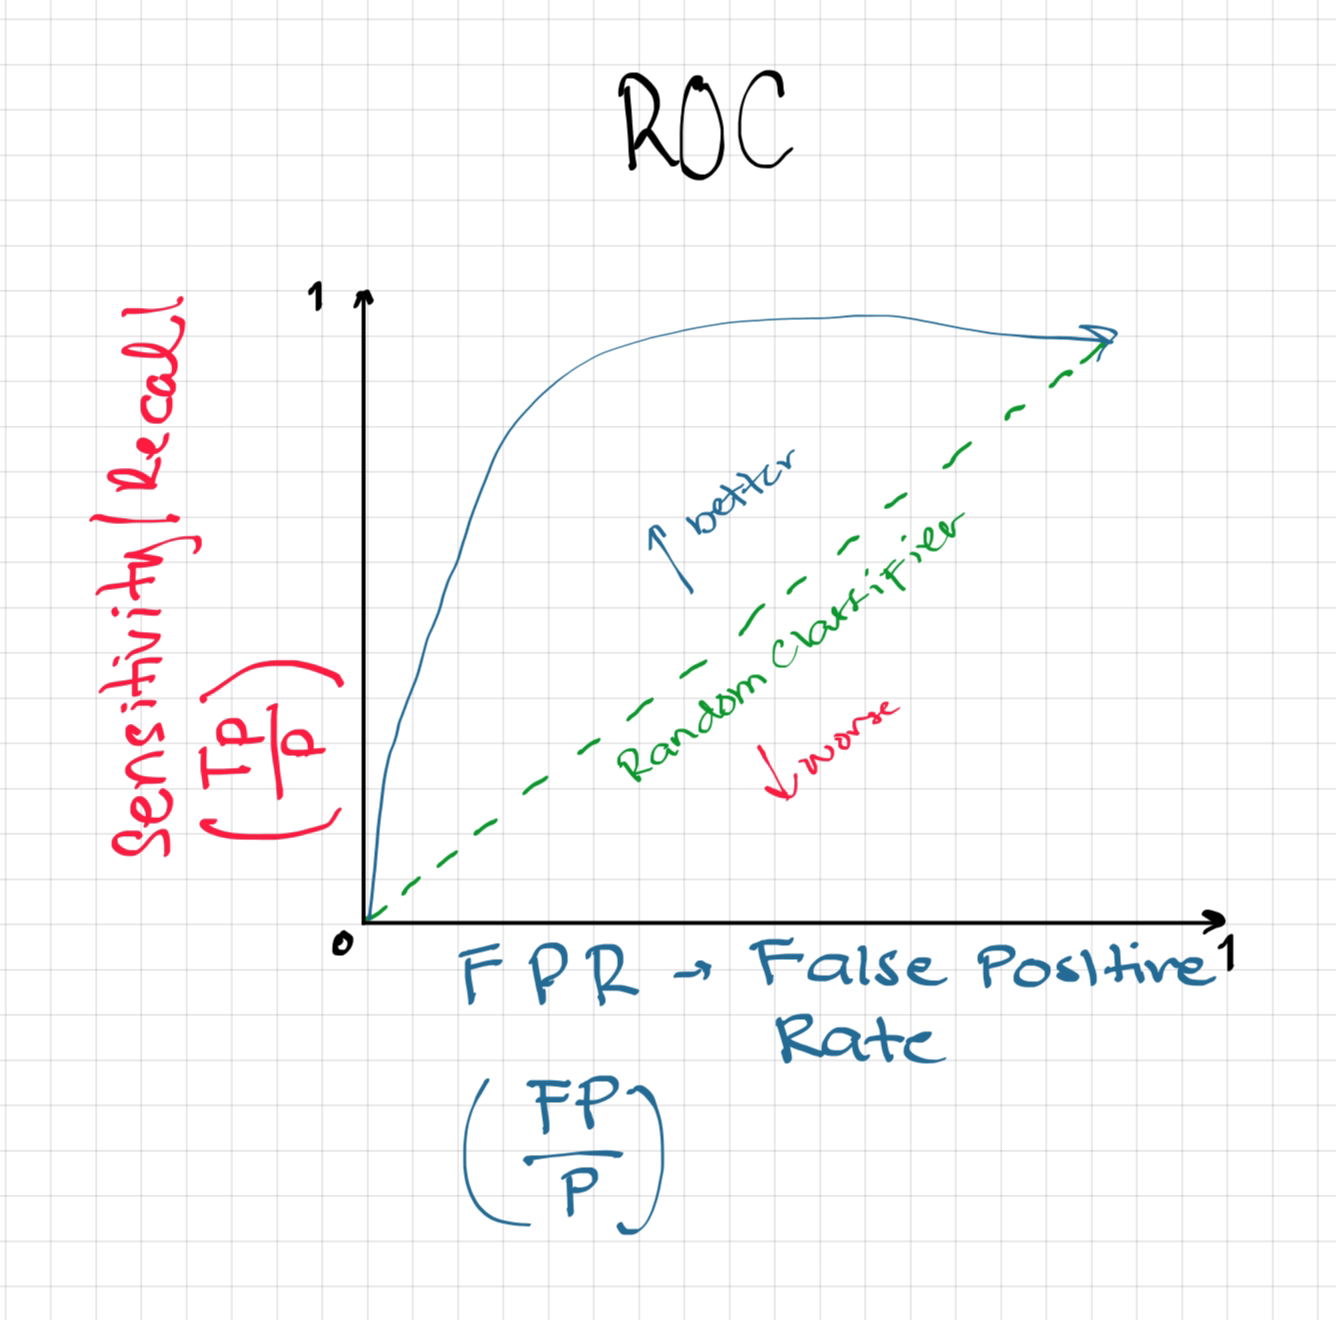
\includegraphics[width=0.8\textwidth]{roc.png} \\ 
    \textbf{Y-axis} : \textbf{Sensitivity/Recall} This is the proportion of correct positive predictions over all predicted positive values. It is computed by getting the True postives over all positive predictions \\ 
    \textbf{X-axis}: \textbf{False Positive Rate} This is the proportion of all predicted positive that were actually false over all positive predictions. It is obtained by getting all the False positives over all predicted positive values. \\ 

    The AUC graph is used to evaluate binary classification models. It plots the sensitivity against the fpr. The closer the AUC value is to 1 the better. 

\easysubproblem{Pick one point on your ROC curve from the previous question. Explain a situation why you would employ this model.}\spc{3} \\ 
If i were to pick a point I'd prefer to be closest to the top left corner because that indicates a higher recall and lower fpr which means the model is good and the auc value is closer to 1.

\intermediatesubproblem{Graph a canonical DET curve and label the axes. Explain very clearly what is measured by the $x$ axis and the $y$ axis. Make sure the DET curve's intersections with the axes is correct.}\spc{7} \\ 
 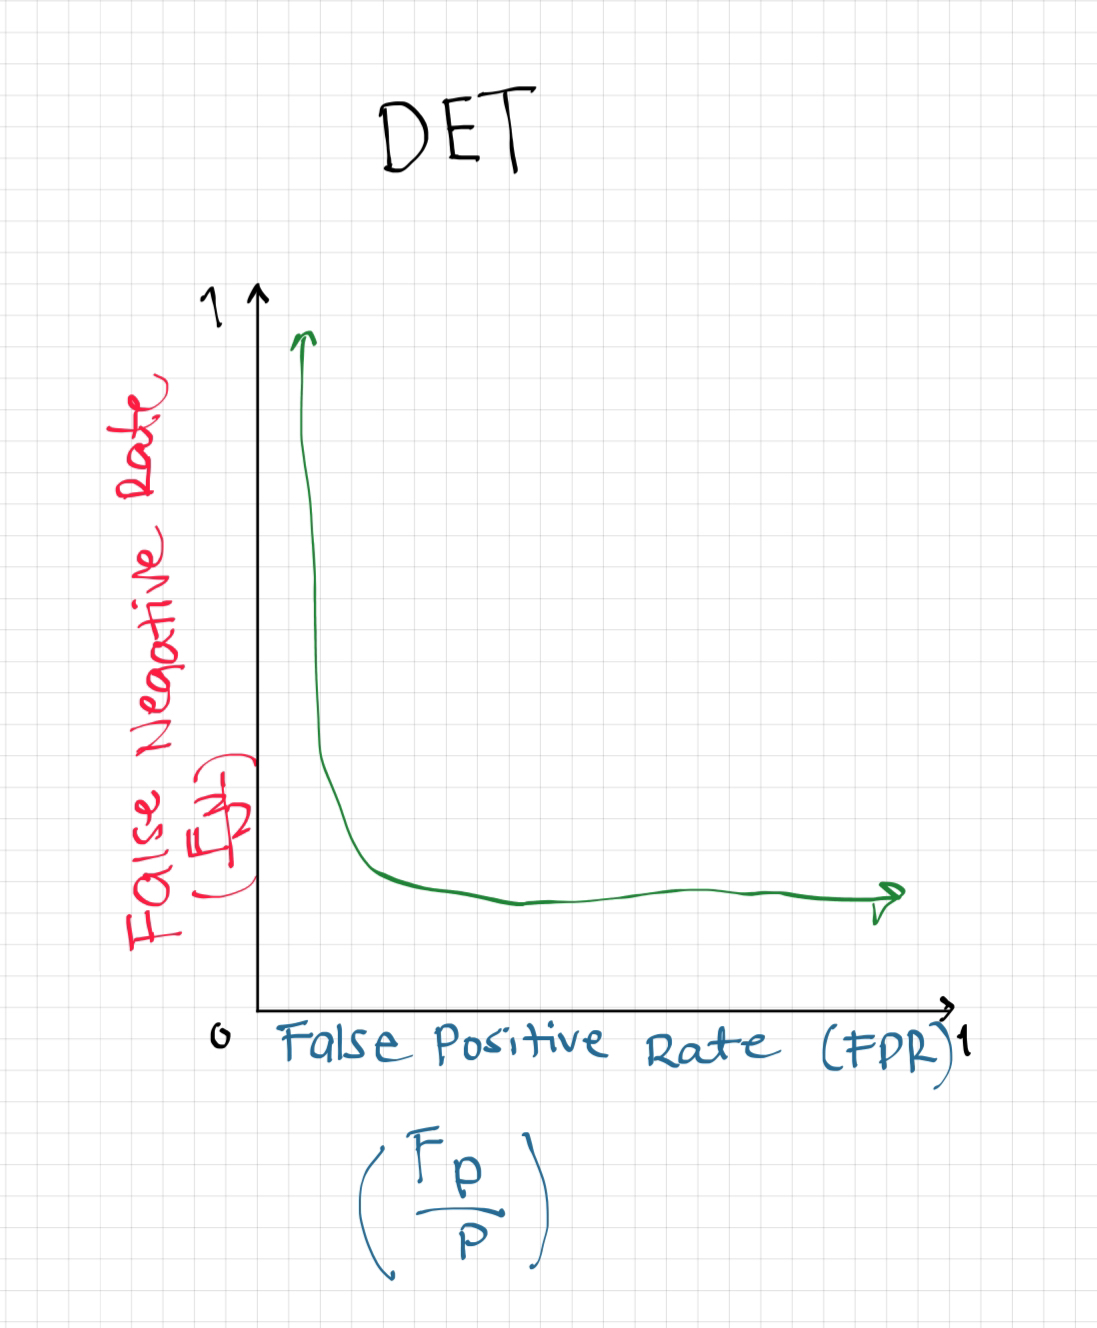
\includegraphics[width=0.8\textwidth]{det.png} \\ 
\textbf{Y-axis} : \textbf{False negative rate} is the proportion of False negatives over all negatives. It is obtained by getting the number of false negatives dividing it over all negative values. 

\textbf{X-axis}: \textbf{False Positive Rate} This is the proportion of all predicted positive that were actually false over all positive predictions. It is obtained by getting all the False positives over all predicted positive values. \\ 

A good model will have low false negative rate and low false positive rate. \\ \\
\easysubproblem{Pick one point on your DET curve from the previous question. Explain a situation why you would employ this model.}\spc{3} \\ 
I would pick a spot on the bottom left where False negative and false positive are both nearing 0. This means the model is barely making mistakes the closer it is to the bottom left corner.

\hardsubproblem{[MA] The line of random guessing on the ROC curve is the diagonal line with slope one extending from the origin. What is the corresponding line of random guessing in the DET curve? This is not easy...}\spc{5}
\end{enumerate} \\ 
\textbf{ANSWER :}In a DET curve, the line of random guessing is a diagonal line extending from the bottom-left corner to the top-right corner. This line represents equal rates of false negatives and false positives, just like random guessing in an ROC curve.  \\

\problem{These are some questions related to bias-variance decomposition. Assume the two assumptions from the notes about the random variable model that produces the $\delta$ values, the error due to ignorance.} \\

\begin{enumerate}
\easysubproblem{Write down (do not derive) the decomposition of MSE for a given $\x_*$ where $\mathbb{D}$ is assumed fixed but the response associated with $\x_*$ is assumed random.}\spc{1} \\ 
\text{MSE}(x^*) = \sigma^2 + (f(x^*) - g(x^*))^2 \\

\easysubproblem{Write down (do not derive) the decomposition of MSE for a given $\x_*$ where the responses in $\mathbb{D}$ is random but the $\X$ matrix is assumed fixed and the response associated with $\x_*$ is assumed random like previously.}\spc{3} \\ 
\text{MSE}(x^*) = \sigma^2 + \text{Bias}[g(x^*)]^2 + \text{Var}[g(x^*)] \\ 

\easysubproblem{Write down (do not derive) the decomposition of MSE for general predictions of a phenomenon where all quantities are considered random.}\spc{3} \\ 
\text{MSE} = \sigma^2 + \mathbb{E}[\text{Bias}[g(x^*)]^2] + \mathbb{E}[\text{Var}[g(x^*)]] \\


\hardsubproblem{Why is it in (a) there is only a \qu{bias} but no \qu{variance} term? Why did the additional source of randomness in (b) spawn the variance term, a new source of error?}\spc{6} \\ \\ 
There is no variance because the dataset is assumed to be fixed. Variance emerges when the dataset changes a model drastically but since the data is assumed to be fixed there is no room for variance. There is bias mainly because either the model we because either we overfit or under-fit.

\intermediatesubproblem{A high bias / low variance algorithm is underfit or overfit?}\spc{-0.5} \\ \\ 
A high bias low variance algorithm is something that is underfit. It can't fit well on what it was trained on and any change in the dataset yields the same or highly similar model. 

\intermediatesubproblem{A low bias / high variance algorithm is underfit or overfit?}\spc{-0.5} \\ 
A low bias high variance algorithm is something that is overfit. It has low bias because it understands the intricacies of the dataset it was trained on a little too well that if the dataset is changed, the model changes drastically. 

\intermediatesubproblem{Explain why bagging reduces MSE for \qu{free} regardless of the algorithm employed.}\spc{6} \\ 
Bagging employs a technique called bootstrapping which samples the dataset with replacement. Each model is then trained on these "different" datasets, leading to slightly different models. When making predictions the errors average out acting as its own form of validation. 

\intermediatesubproblem{Explain why RF reduces MSE atop bagging $M$ trees and specifically mention the target that it attacks in the MSE decomposition formula and why it's able to reduce that target.}\spc{5} \\ \\ 
Random forrest is an ensembling method that utilizes alot of decision trees under the hood. Decision trees is an example of a low bias high variance algorithm due to its ability to fit onto anything. Given that a random forrest deploys a lot of decision trees which are all trained with different subsets of the features within the dataset reducing the variance of the forrest all together while reducing bias for free. 

\hardsubproblem{When can RF lose to bagging $M$ trees? Hint: think hyperparameter choice.}\spc{5} \\ 
Random forrest looses to bagged trees if the features for each tree are still highly correlated. If random forrest uses too features per split it leads to high correlation defeating the purpose of random forrest.
\end{enumerate} 


%\problem{These are some questions related to correlation-causation and interpretation of OLS coefficients.}
%
%\begin{enumerate}
%\easysubproblem{Consider a fitted OLS model for y with features $x_1$, $x_2$, \ldots, $x_p$. Provide the most correct interpretation of the quantity $b_1$ you can.}\spc{6}
%
%
%\easysubproblem{If $x$ and $y$ are correlated but their relationship isn't causal, draw a diagram below that includes $z$.}\spc{6}
%
%\easysubproblem{To show that $x$ is causal for $y$, what specifically has to be demonstrated? Answer with a couple of sentences.}\spc{4}
%
%\intermediatesubproblem{If we fit a model for y using $x_1$, $x_2$, \ldots, $x_7$, provide an example real-world illustration of the causal diagram for $y$ including the $z_1$, $z_2$, $z_3$.}\spc{5}
%
%
%\end{enumerate}
%
%

\newpage
\problem{These are some questions related to missingness.}

\begin{enumerate}
\easysubproblem{[MA] What are the three missing data mechanisms? Provide an example when each occurs (i.e., a real world situation). We didn't really cover this in class so I'm making it a MA question only. This concept will NOT be on the exam.}\spc{4} \\ 

\textbf{Missing Completely at Random (MCAR):}  \\
\textbf{Definition}: Data missing for no particular reason.\\
\textbf{Example}: A survey response is lost in the mail. \\ 

\textbf{Missing at Random (MAR):} \\
\textbf{Definition}: Data missing due to some observed data, but not the missing data itself.\\
\textbf{Example}: Higher-income people are less likely to report their income in a survey, but their age and education level are known. \\ 

\textbf{Missing Not at Random (MNAR):} \\
\textbf{Definition}: Data missing due to the value of the missing data itself. \\
\textbf{Example}: People with very high medical expenses are less likely to report their expenses in a health survey. \\

\easysubproblem{Why is listwise-deletion a \textit{terrible} idea to employ in your $\mathbb{D}$ when doing supervised learning?}\spc{3} \\ 
There are multiple reasons why list-wise deletion is bad because data is the most important aspect of supervised learning. The missingness of a value may be an indicator itself like a student who has no grades may mean that they never attend class. There are also imputation techniques that handle missingness. 

\easysubproblem{Why is it good practice to augment $\mathbb{D}$ to include missingness dummies? In other words, why would this increase oos predictive accuracy?}\spc{4} \\ 
Because when there are missing values it could have some sort of predictive power. Data being missing may mean something. Separating it into its own level/class allows us to handle the missing data and use it to our advantage and allowing us to increase oos predictive accuracy because when missing data is augmented it is rendered to be useful. 

\easysubproblem{To impute missing values in $\mathbb{D}$, what is a good default strategy and why?}\spc{5} \\ The greedy approach is to use the mean or mode to fill in missing data with in a column. A smarter approach which could be utilized is by interpolation. This is done by making a predictive model for each feature that has missingness, even including the target variable as a predictor.. An example algorithm that handles missingness is \textbf{missForrest}

\end{enumerate}
%
%\problem{These are some questions related to lasso, ridge and the elastic net.}
%
%\begin{enumerate}
%\easysubproblem{Write down the objective function to be minimized for ridge. Use $\lambda$ as the hyperparameter.}\spc{2}
%
%\easysubproblem{Write down the objective function to be minimized for lasso. Use $\lambda$ as the hyperparameter.}\spc{3}
%
%\easysubproblem{We spoke in class about when ridge and lasso are employed. Based on this discussion, why should we restrict $\lambda > 0$?}\spc{3}
%
%\intermediatesubproblem{Why is lasso sometimes used a preprocessing step to remove variables that likely are not important in predicting the response?}\spc{3}
%
%
%\easysubproblem{Assume $\X$ is orthonormal. One can derive $\b_{\text{lasso}}$ in closed form. Copy the answer from the wikipedia page. Compare $\b_{\text{lasso}}$ to $\b_{\text{OLS}}$.}\spc{8}
%
%\intermediatesubproblem{Write down the objective function to be minimized for the elastic net. Use $\alpha$ and $\lambda$ as the hyperparameters.}\spc{3}
%
%\easysubproblem{We spoke in class about the concept of the elastic net. Based on this discussion, why should we restrict $\alpha \in (0, 1)$?}\spc{3}
%
%\end{enumerate}
\problem{These are some questions related to gradient boosting. The final gradient boosted model after $M$ iterations is denoted $G_M$ which can be written in a number of equivalent ways (see below). The $g_t$'s denote constituent models and the $G_t$'s denote partial sums of the constituent models up to iteration number $t$. The constituent models are \qu{steps in functional steps} which have a step size $\eta$ and a direction component denoted $\tilde{g}_t$. The directional component is the base learner $\mathcal{A}$ fit to the negative gradient of the objective function $L$ which measures how close the current predictions are to the real values of the responses:

\beqn
G_M &=& G_{M-1} + g_M \\
&=& g_0 + g_1 + \ldots + g_M \\
&=& g_0 + \eta \tilde{g}_1 + \ldots + \eta \tilde{g}_M \\
&=& g_0 + \eta \mathcal{A}\parens{\left<\X, -\nabla L(\y, \yhat_1)\right>, \mathcal{H}} + \ldots + \eta \mathcal{A}\parens{\left<\X, -\nabla L(\y, \yhat_M)\right>, \mathcal{H}} \\
&=& g_0 + \eta \mathcal{A}\parens{\left<\X, -\nabla L(\y, g_1(\X))\right>, \mathcal{H}} + \ldots + \eta \mathcal{A}\parens{\left<\X, -\nabla L(\y, g_M(\X))\right>, \mathcal{H}} 
\eeqn}

\begin{enumerate}
\easysubproblem{From a perspective of only multivariable calculus, explain gradient descent and why it's a good idea to find the minimum inputs for an objective function $L$ (in English).}\spc{2.5} \\ 
Gradient descent is a method for optimizing and finding the minimum of an objective function. It works by repeatedly moving in the direction of the negative gradient (the steepest downward slope) of the function. By doing so, it identifies the input values that minimize the function. This process is crucial because lowering the objective function typically leads to better model performance, fewer errors, and higher accuracy. 

\newpage
\easysubproblem{Write the mathematical steps of gradient boosting for supervised learning below. Use $L$ for the objective function to keep the procedure general. Use notation found in the problem header. 
}\spc{8} \\ \\ 
\begin{enumerate}
    \item \textbf{Initialize the model}:
    \[
    G_0 = g_0
    \]

    \item \textbf{Iterative procedure for \( M \) steps}:
    \[
    G_M = G_{M-1} + g_M
    \]

    \item \textbf{Decompose \( G_M \)}:
    \[
    G_M = g_0 + g_1 + \cdots + g_M
    \]

    \item \textbf{Express \( g_M \) in terms of the learning rate \( \eta \) and the gradients \( \tilde{g} \)}:
    \[
    G_M = g_0 + \eta \tilde{g}_1 + \cdots + \eta \tilde{g}_M
    \]

    \item \textbf{Express the gradients \( \tilde{g} \) as functions of the inner products and the objective function \( L \)}:
    \[
    G_M = g_0 + \eta A (\langle X, -\nabla L(y, \hat{y}_1) \rangle, H) + \cdots + \eta A (\langle X, -\nabla L(y, \hat{y}_M) \rangle, H)
    \]

    \item \textbf{Finally, express the gradients in terms of the current model predictions}:
    \[
    G_M = g_0 + \eta A (\langle X, -\nabla L(y, g_1(X)) \rangle, H) + \cdots + \eta A (\langle X, -\nabla L(y, g_M(X)) \rangle, H)
    \]
\end{enumerate}

\easysubproblem{For regression, what is $g_0(\x)$?}\spc{1} \\ 
g_0(x) = \hat{y}_0 = \bar{y}_i \\

\easysubproblem{For probability estimation for binary response, what is $g_0(\x)$?}\spc{1} \\  g_0(x) = \ln \left( \frac{\hat{p}_i}{1 - \hat{p}_i} \right) \\


\intermediatesubproblem{What are all the hyperparameters of gradient boosting? There are more than just two.}\spc{3} \\ 

\mathbf{\eta} (learning rate), m (number of trees), N_0 (minimum samples per leaf, L (max depth of trees), Subsample, \\Maximum Features, Loss function, \\Minimum samples per split, Regularization parameters, random state. \\

 

\easysubproblem{For regression, rederive the negative gradient of the objective function $L$.}\spc{2} \\ 
\begin{itemize}
    \item For regression, consider \( L(\mathbf{y}, \tilde{\mathbf{y}}) = \frac{1}{2N} \sum_i (\tilde{y}_i - y_i)^2 \Rightarrow - \nabla L(\mathbf{y}, \tilde{\mathbf{y}}) \):
    \[
    - \nabla L(\mathbf{y}, \tilde{\mathbf{y}}) = 
    \begin{bmatrix}
        2(y_1 - \hat{y}_1) \\
        2(y_2 - \hat{y}_2) \\
        \vdots \\
        2(y_n - \hat{y}_n)
    \end{bmatrix}
    = 2(\mathbf{y} - \hat{\mathbf{y}}) \approx -2\eta A(\langle X, X \rangle, H)
    \]
\end{itemize}
\\

\easysubproblem{For probability estimation for binary response, rederive the negative gradient of the objective function $L$.}\spc{12} \\ 
\begin{itemize}
    \item \textbf{Probability estimation for binary response}:
    \begin{itemize}
        \item Recall the likelihood function:
        \[
        \prod_i \hat{p}_i^{y_i} (1 - \hat{p}_i)^{1 - y_i}
        \]
        
        \item Reparameterize with log-odds: let \( \tilde{y}_i = \ln \left( \frac{\hat{p}_i}{1 - \hat{p}_i} \right) \) \( \iff \) \( \hat{p}_i = \frac{e^{\tilde{y}_i}}{1 + e^{\tilde{y}_i}} \)
        
        \item The likelihood function now becomes:
        \[
        \prod_i \left( \frac{e^{\tilde{y}_i}}{1 + e^{\tilde{y}_i}} \right)^{y_i} \left( \frac{1}{1 + e^{\tilde{y}_i}} \right)^{1 - y_i} = \prod_i \left( \frac{e^{\tilde{y}_i y_i}}{(1 + e^{\tilde{y}_i})} \right)
        \]
        
        \item Now we have:
        \[
        - \nabla L(\mathbf{y}, \tilde{\mathbf{y}}) = 
        \begin{bmatrix}
            \frac{y_1 - \hat{p}_1}{1 - \hat{p}_1} \\
            \frac{y_2 - \hat{p}_2}{1 - \hat{p}_2} \\
            \vdots \\
            \frac{y_n - \hat{p}_n}{1 - \hat{p}_n}
        \end{bmatrix}
        = \mathbf{y} - \hat{\mathbf{p}}
        \]
    \end{itemize}
\end{itemize}

\hardsubproblem{For probability estimation for binary response scenarios, what is the unit of the output $G_M(\x_\star)$?}\spc{2} \\ 
The result is in Log odds 

\easysubproblem{For the base learner algorithm $\mathcal{A}$, why is it a good idea to use shallow CART (which is the recommended default)?}\spc{2} \\ 
Shallow trees are less likely to overfit

\hardsubproblem{For the base learner algorithm $\mathcal{A}$, why is it a bad idea to use deep CART?}\spc{2} \\ 
Deep trees become overly specific in the dataset they are trained. Since they are deep they are highly likely to overfit.

\hardsubproblem{For the base learner algorithm $\mathcal{A}$, why is it a bad idea to use OLS for regression (or logistic regression for probability estimation for binary response)?}\spc{2} \\ 
OLS fail to describe situations where the data has a non-linear relationship. Unlike trees that could be simple but is able to fit complex data.

\hardsubproblem{If $M$ is very, very large, what is the risk in using gradient boosting even using shallow CART as the base learner (the recommended default)?}\spc{2} \\ 
If M becomes exessively large the model may end up picking up the noise and overfitting. 

\hardsubproblem{If $\eta$ is very, very large but $M$ reasonably correctly chosen, what is the risk in using gradient boosting even using shallow CART as the base learner (the recommended default)?}\spc{2} \\ 
If $\eta$ is very large at each step it may take major leaps and missing the optimal solutions.

\end{enumerate}




\end{document}






